\documentclass[12pt, twoside]{article}
\usepackage[francais]{babel}
\usepackage[T1]{fontenc}
\usepackage[latin1]{inputenc}
\usepackage[left=7mm, right=7mm, top=7mm, bottom=7mm]{geometry}
\usepackage{float}
\usepackage{graphicx}
\usepackage{array}
\usepackage{multirow}
\usepackage{amsmath,amssymb,mathrsfs}
\usepackage{soul}
\usepackage{textcomp}
\usepackage{eurosym}
 \usepackage{variations}
\usepackage{tabvar}


\pagestyle{empty}

\begin{document}




\section*{\center{Devoir maison 4}}


\bigskip



 
 
\fbox{

\begin{minipage}{18cm}
\textit{Devoir � rendre pour le \textbf{\ldots \ldots \ldots \ldots \ldots f�vrier
2015}.
La pr�sentation et la clart� sont not�es sur 1 point. Tous les calculs doivent
�tre �crits et pos�s.}
\end{minipage}
}


\bigskip


\ul{Exercice 1}: (\textit{4 points}) 

\enskip

\begin{tabular}{ccc}
\textbf{Poser} et effectuer: \quad & a) $8,057 + 79,4$ \qquad \qquad  & \qquad
\qquad $b) 240-8,09$ \\

\quad & \quad & \quad \\

\quad & c) $3,67 \times 2,9$ \qquad \qquad  & \qquad \qquad  d) $14,08 \times
5,2$
\\
\end{tabular}
  



\bigskip

\medskip

 
 \ul{Exercice 2}: (\textit{3 points})
 R�soudre les probl�mes suivants (pensez � marquer vos calculs).
 
 \begin{enumerate}
   \item Un marchand d'oeufs revient du march� avec 175 oeufs. Il en a vendu
   237. Combien d'oeufs avait-il en se rendant au march�?
   \item Mourad a 7 ans de plus que Nicolas. Nicolas a 11 ans. Quel est l'�ge de
   Mourad?
   \item Julien a 4 \euro. Son ami Maxime a 1,3 \euro de moins que lui. Combien
   ont-ils � eux deux?
 \end{enumerate}
  
 
 \bigskip
 
 
 \medskip
 
 \ul{Exercice 3}: (\textit{3,5 points})
 
 \begin{enumerate}
   \item \textbf{Poser} et effectuer:
   
   \begin{enumerate}
     \item 
    7 h 28 min + 11 h 43 min 
   \item 17 h 23 min - 4 h 47 min
   \end{enumerate}
   \item Titouan est artisan peintre. Aujourd'hui, il a pass� 3 heures et 45
   minutes � enlever la vieille tapisserie. Ensuite, il a mit 50 minutes pour
   peindre le plafond. Enfin, poser la nouvelle tapisserie l'a occup� pendant
   5 h 20 min. Combien de temps Titouan a-t-il travaill�?
 \end{enumerate}
 
 \bigskip
 
 \medskip
 
 
 \ul{Exercice 4}: (\textit{2,5 points})
 
 \enskip
 
 Xavier a encore assez d'essence dans son scooter pour faire 28 km. Il va
 au march� � 9,8 km. Puis il part voir son fr�re � 4,2 km et r�cup�re un livre
 � la librairie qui se situe � 4,9 km. Ensuite, il rentre chez lui � 14,8 km.
 
 En utilisant les ordres de grandeur, dire si Xavier doit remettre ou non de
 l'essence dans son scooter. Expliquer.
 
 \bigskip
 
 
 \medskip
 
 
\ul{Exercice 5}: (\textit{2,5 points})


\begin{tabular}{cc}

\begin{minipage}{10cm}
Jacques et Patricia ont install� leur tente pour cinq jours au camping du
Moulin. Ils sont accompagn�s de leurs enfants, Gabriel qui a 15 ans et Sarah
qui a 11 ans ainsi que de leur chien Fido. 

Combien vont-ils payer leur s�jour?
\end{minipage}
&

\begin{minipage}{8cm}

\quad \quad  
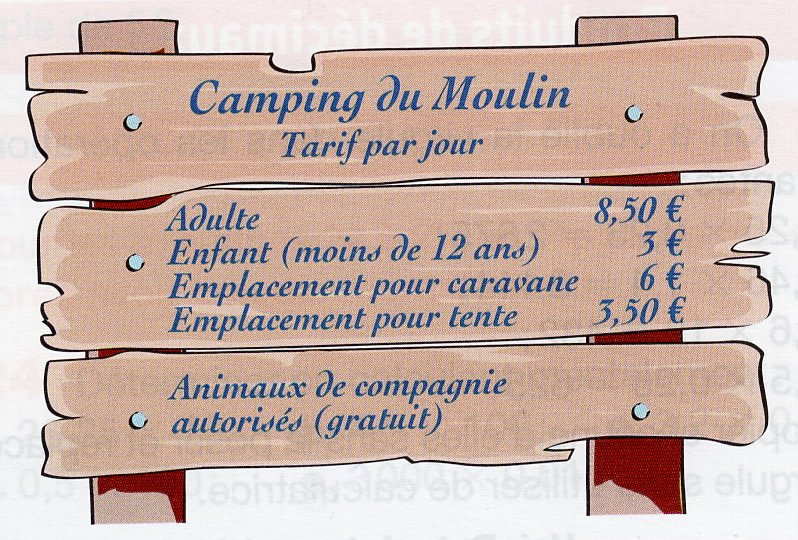
\includegraphics[width=7cm]{images/camping.jpg}
\end{minipage}

\end{tabular}

\medskip


\bigskip


\ul{Exercice 6}: (\textit{3,5 points})


\enskip

Sur un march� de Provence, j'ach�te 0,350 kg d'olives noires � 12,40 \euro
\thinspace le kg et 0,840 kg d'olives vertes au poivron � 17,50 \euro
\thinspace le kg. Je donne un billet de 20 \euro \thinspace � la commer�ante.


Combien va-t-elle me rendre?
\end{document}
